%\documentclass[fleqn,10pt]{book}  % fleqn left alligns all equations. 
\documentclass[altfont]{uiophd}
\usepackage[usenames,dvipsnames,svgnames]{xcolor}			
\usepackage{titlesec}		% Can change properties of sections, such as color. 
\usepackage{fancyhdr}		% Adds customizable headers and footers. 
\usepackage{titletoc}		% Adds small toc lists. 
\usepackage{hyperref}
\usepackage{graphicx}
\usepackage{bm,upgreek,textcomp} % Some extra signs and other fonts.
\usepackage[
	backend=bibtex,
	style=numeric,
	sorting=none,
	url=false,
	doi=false,
	isbn=false, 
	maxcitenames=2,
]{biblatex}
%\usepackage{cite}
%\bibliography{master}
\addbibresource{master.bib}
\AtEveryBibitem{\clearfield{month}}
\AtEveryBibitem{\clearfield{day}}
\AtEveryCitekey{\clearfield{month}}

% Use ampersand "&" instead of "and". 
\renewcommand*{\finalnamedelim}{%
  \ifnumgreater{\value{liststop}}{2}{\finalandcomma}{}%
  \addspace\&\space}

% Paper properties. 
\pagestyle{fancy}
% Removes the header bar and text.
\renewcommand{\headrulewidth}{0pt}
\fancyhead{}

% Custom colors.
\definecolor{viridis_01}{rgb}{0.267004, 0.048740, 0.329415}
\definecolor{viridis_02}{rgb}{0.190631, 0.407061, 0.556089}
\definecolor{viridis_03}{rgb}{0.208030, 0.718701, 0.472873}
\definecolor{viridis_04}{rgb}{0.993248, 0.906157, 0.143936}

\titleformat{\section}
{\color{viridis_02}\Large\bfseries}
{\color{viridis_02}\thesection}{1em}{} 		

\titleformat{\subsection}
{\color{viridis_02}\large\bfseries}	
{\color{viridis_02}\thesubsection}{1em}{}

% Change section formatting.
\titleformat{\chapter}[hang] 				
{\bfseries\Huge} 	
{\color{viridis_01}\thechapter\hspace{20pt}\rule[-3pt]{2pt}{23pt}\hspace{10pt}}
{0.5ex} 			
{\color{viridis_01}} 	
[
	%\small
	%\startcontents
	%\printcontents{}{1}{\setcounter{tocdepth}{1}}
]		

% Remap \cite to \mycite.
\DeclareCiteCommand{\mycite}
  {\usebibmacro{prenote}}
  {%
    \printnames{labelname}
    \usebibmacro{date} %
    [\usebibmacro{cite}] %
  }
  {\multicitedelim}
  {\usebibmacro{postnote}}
  
\renewcommand{\cite}[1]{\mycite{#1}}

% Remap \citetitle to \mycitetitle.
\DeclareCiteCommand{\mycitetitle}
  {\usebibmacro{prenote}}
  {%
    \thefield{title} 
    \usebibmacro{date} %
    [\usebibmacro{cite}] %
  }
  {\multicitedelim}
  {\usebibmacro{postnote}}
  
\renewcommand{\citetitle}[1]{\mycitetitle{#1}}

% Remap \textcite to \mytextcite
\DeclareCiteCommand{\mytextcite}
  {\usebibmacro{prenote}}
  {%
    \printnames{labelname}
    (\usebibmacro{date})%
  }
  {\multicitedelim}
  {\usebibmacro{postnote}}
  
\renewcommand{\textcite}[1]{\mytextcite{#1}}

% Change the color of every citation.
\AtEveryCite{\color{viridis_03}}

% Hyperlink colors. 
\hypersetup{
	colorlinks,
	citecolor=viridis_03,
	filecolor=black,
	linkcolor=black,
	urlcolor=black
}

\begin{document}

\chapter*{Abstract}
(Abstracts do not include sources, but are here for the purpose of notes.) \\

\noindent
The physical processes that creates electrical signals in neurons are well understood, 
but how the signals are processed into actions and thoughts has yet to 
receive a scientifically robust answer
(add more sources) 
\cite{sterratt2011principles}. 
Cell type classification is of high importance because the function of different 
neurons is still largely a mystery. 

\setcounter{tocdepth}{1}
\startcontents
\tableofcontents

\chapter{Introduction}
Introduce the topic, the problem and how the problem is being solved. 

Since 
the conception of neuroscience the neurons function have been studied on many levels
and with many perspectives, 
from a single neuron level to networks of neurons with chemistry, physics, medicine
and psychology to name some. 


\chapter{Theory}
Each section introduces topics that are referenced frequently in the article. 
At the end of each section there is a background subsection. 
These subsections contain information
about the current state of research on the topic and previous work. 
%Introduce topics so a bachelor student can understand. 

\vspace{1em} 
\startcontents
\printcontents{}{1}{\setcounter{tocdepth}{2}}
  
\section{The Neuron}
Neurons are excitiable brain cells capable of transmitting voltage changes across its 
structure which again can excite other neurons. These sharp voltage changes are called 
action potentials and when a neuron creates an action potential it is said to "fire".

(TODO: Add picture of neuron and explain all the parts.)

(TODO: Add more, citations.)

Topic to mention:
Neuron cell types, pyramidal neurons, basket neurons interneurons, what 
are they. The term "morphology". Intracellular also referred to as membrane potential.
Subcortical. Se hemalainen p.421. for a good summary. What is transmembrane current. 
Impulse. Apical dendrites. Grey matter. Spines. Synapses. Quiescent neuron.


\subsection*{Background}
The physical processes in and around neurons are well understood in comparison
to the function they serve. 
The consensus is that the basic function of a neuron is to receive and send 
action potentials and that action potentials are 
responsible for all cognitive functions.
What information is transmitted in the action potentials and how 
the information is processed is still under much research.  


\section{Action Potentials}
Describe how actionpotentials are created. 

\subsection*{Background}
Write about hodking and huxley. \cite{hodgkin_quantitative_1952}

\section{Neuronal Models}
There are multiple models for neurons, some of the main groups are 
point models and compartmental models. List many models?
Multi-compartmental models 
can be useful to understand the processing of neurons with
complex morphological structures
\cite{sterratt_principles_2011}. 
\subsection*{Background}
\cite{hodgkin_quantitative_1952} \cite{connor_prediction_1971} \cite{sterratt_principles_2011}

\section{Electrodes}


\section{Calculating Extracellular Potential}
The extracellular potential is the electric potential generated from the transmembrane
currents in the neurons. When a neuron fires this can be seen from the extracellular
potential, which will have a spike which is similar to the intracellular spike.

The extracellular potential can be calculated
using Maxwell's eqations and the continuity equation if the spatial
distribution (morphology) of transmembrane currents and the extracellular conductivity
is known. 
This
information can be hard to obtain in vitro, but if these
values are obtained either using neuron models
or physical recordings the extracellular potental is in theory 
easy to calculate in a computer. \\

\noindent
To make calculation easier, some assumptions are made: 
\begin{enumerate}
	\item The permeability $\mu $ of 
	the extracellular medium is the same as that of vacuum $\mu_0$.
	\item Assume a quasistatic approximation which lets the $\partial E/\partial t$
	be ignored and as source terms. Link to appendix for proof. 
\end{enumerate}
Forward problem = calculate the potential from the current source, inverse problem is used
in magnetoenchephalography (important).
The amplitude of a spike in the
extracellular potential is usually in the magnintude of
$< 200 \upmu$V.  
The noise of electrodes vary, but can be as much as $20 \upmu$V. 
This limits the range electrodes can record from. 

The currents sum to zero, while the spike is very visible, there are many small currents
in the dendrites with opposite current. 
(\cite{hamalainen_magnetoencephalography-_1993})

The extracellular spike width tend to increase with distance from soma because of the
neuronal morphology. 
This article used a passive neuron model with different morphologies to show
that the spike width increases with distance to soma. The spike amplitude also
decreases with distance to soma and seems to follow a power law. 
(\cite{pettersen_amplitude_2008} \hspace{-3pt}).

The shape of extracellular spikes are mainly depedent on the membrane currents
and the morphology of the cell. 
Some of the effects from the morphology of the cell are increased spike width and
decreased amplitude from distance to soma. 

Many things here from around page 245. 
When the conductivity $\sigma$ and the current generators are know, Maxwell's
equations and the continuity equation equation can be used to calculate the electric
field $E$ and magnetic field $B$. (TODO: Copied text)
(\cite{hamalainen_magnetoencephalography-_1993})

\subsection*{Background}
Electric potential from neurons can either be obtained 
by measuring the membrane potential or measured from the the extracellular
medium. 
%Recording the membrane potential is easier to interpret but harder to execute 
%while 
%extracellular recordings are harder to interpret but easier to execute. 
Recording is usually done using electrodes, this makes recording the membrane potential
more challenging than recording from the extracellular medium as the electrode
has to be very close or inside the cell. 
At the time of writing  
recording the membrane potential of a concious subject is nearly impossible,
this makes understanding extracellular potentials vital for current research. 
As such it is useful to know the physical origin of the extracellular potential. 

Early calculations was done by Rall 1962 investigating 
the interaction between action potentials and synapes using cylinders
as the current source. (TODO: Read article, make more understandble.)
Holt and Koch 1999 added comparmental models to reconstruct pyramidal neurons. 

\section{Neuron \& LFPy }
LFPy is a Python module that uses Neuron and the mentioned methods to calculate the 
electric field outside the neuron. 
\cite{linden_lfpy:_2013}
\subsection*{Background}

\section{Cell Type Classification}
\subsection*{Background}
It was early observed that the shape of action potentials are different for 
individual neurons and it has been suggested that action potentials
can be used to identify classes of neurons. This the main focus of this article. 
(Use this source?
\cite{mountcastle_cortical_1969}.




\section{Allen Cell Types Database}
The Allen Brain Institute have gather individual neuron data from lateral geniculate
nucleus (LGN) and primary visual cortex (V1) of young laboratory mice. 
The data's main categories are electrophysiology, morphology and modeling
.
With the morphological data the extracellular potential can be calculated given
a model for the transmembrane currents. 
\citetitle{_allen_2015}
\subsection*{Background}


\chapter{Methods}
\vspace{1em} 
\startcontents
\printcontents{}{1}{\setcounter{tocdepth}{3}}

\section{Pettersen \& Einevoll (2008) Reproduction}
\textcite{pettersen_amplitude_2008} shows some features of extracellular 
spike modulation and
results presented here are comparable to results in the paper. 
See chapter something for extracellular spike modulation.
(\cite{pettersen_amplitude_2008}) \\

Write more about the connor stevens model.

\subsection{Simulation}
\emph{Cell:}
Used the \textcite{mainen_influence_1996} cell with a passive model, 
the same model used in the \textcite{pettersen_amplitude_2008}. 
The cell was rotated using PCA (principal component analysis) on the compartment
positions
so that the first component was paralell to y-axis while the second component
was paralell to the x-axis. This rotates the cell so most of the dendrites are along
the y and x-axis. (TODO: show the morphology of the neuron)\\

\noindent\emph{Spike Generation:}
An action potental was generated using the Connor-Stevens model 
(\cite{connor_prediction_1971}, \cite{connor_neural_1977}) 
using the same parameters as \textcite{dayan_theoretical_2001}. 
This had an amplitude of $107.6mV$ from baseline with the peak at $48.21mV$. 
These values are similar (TODO: how similar?) to \textcite{dayan_theoretical_2001}, but not
with \textcite{pettersen_amplitude_2008} which had an amplitude of 
$83mV$ from baseline. To compensate for the difference the action potental was 
normalized to $83mV$ manually (Figure \ref{fig:3_1_soma_mem}).
\\

\begin{figure}[h]
\centering
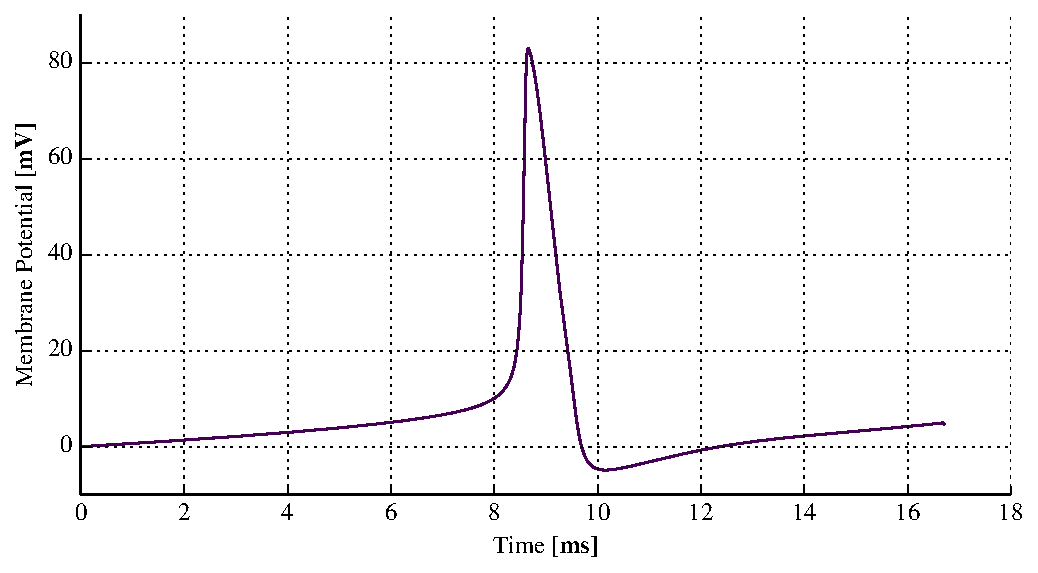
\includegraphics[width=1\textwidth]{images/3_methods/3_1_reproduction/soma_mem.pdf}
\caption{Soma membrane voltage. }
\label{fig:3_1_soma_mem}
\end{figure}


\noindent\emph{Parameters:}
Parameters are the same as \textcite{pettersen_amplitude_2008} and 
\textcite{dayan_theoretical_2001} . Membrane resistance 
$R_m = 3\cdot10^4\Omega /cm^2$, membrane capacitance $C_m=1\mu F / cm^2$, 
axial resistance $R_a = 150\Omega/cm^2$, time resolution $dt=2^{-6}ms$. 
The reversal potential was set to zero. The action potental was imposed in all
soma sections using the "play" vector function in Neuron.
\\

\noindent\emph{Electrode Positions:}
Recording sites were placed in the xz plane at 11 linearly spaced 
positions along 36 lines with equal 
angular spacing. (TODO: Show the electrode positions.) 
\\


\noindent\emph{Spike Width \& Amplitude:}
A baseline was set as the value at the start of the signal. 
Amplitude was calculated as the difference between maximum absolute value and the
baseline.
The spike width was calculated at half width at maximum amplitude. 

Spike width was recorded at $0.5625 ms$ for $dt=2\cdot10^{-5}$, similar to 
$0.55ms$ from \textcite{pettersen_amplitude_2008}. When increasing the
resolution to $dt=2\cdot10^{-6}ms$ the spike width rose to $0.625ms$. 


\subsection{Results}
The action potental that was used in \textcite{pettersen_amplitude_2008} 
is similar to the one used here.  The fourier specter is displayed in
Figure \ref{fig:3_1_fourier}. The graph displayed in the paper and 
the one shown here are nearly identical. 
(TODO: Rewrite, be more spsific here?) \\

\begin{figure}[thp]
\centering
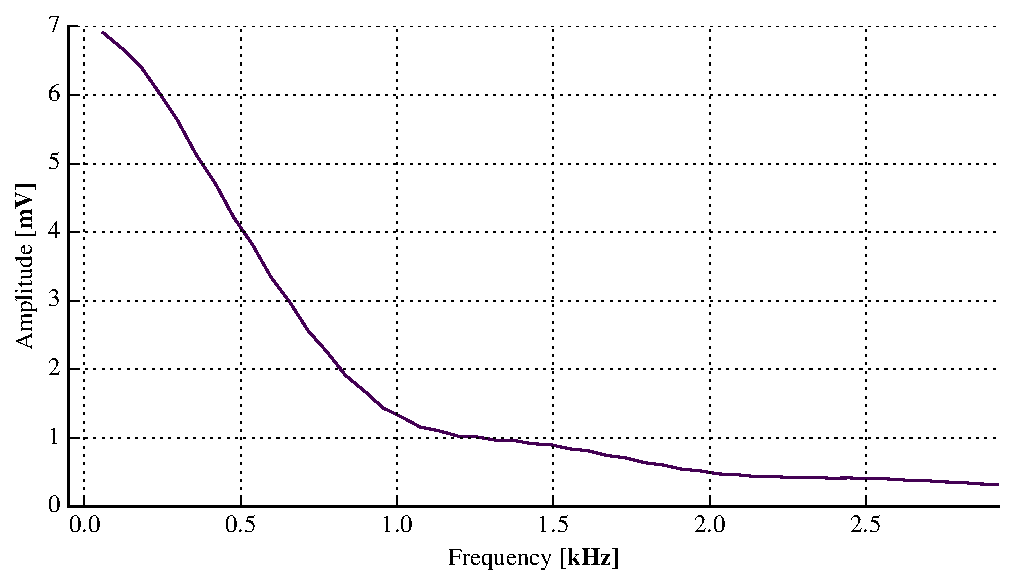
\includegraphics[width=\textwidth]{images/3_methods/3_1_reproduction/soma_mem_fourier.pdf}
\caption{Frequency specter of simulated somatic membrane potential.}
\label{fig:3_1_fourier}
\end{figure}

The spike width increases with the distance from soma as seen in 
Figure \ref{fig:3_1_spike_width}. These results are 
lower than the widths reported in \textcite{pettersen_amplitude_2008}.
(Use more time on editing the Connor-Stevens model to come closer to 
an max.amplitude on 20mV?).   

Sudden changes in spike width was experienced with increased distance from
soma. Above $200\mu V$ the
spikes shapes are not well defined. 
This was also reported in \textcite{pettersen_amplitude_2008}.\\

\begin{figure}[thp]
\centering
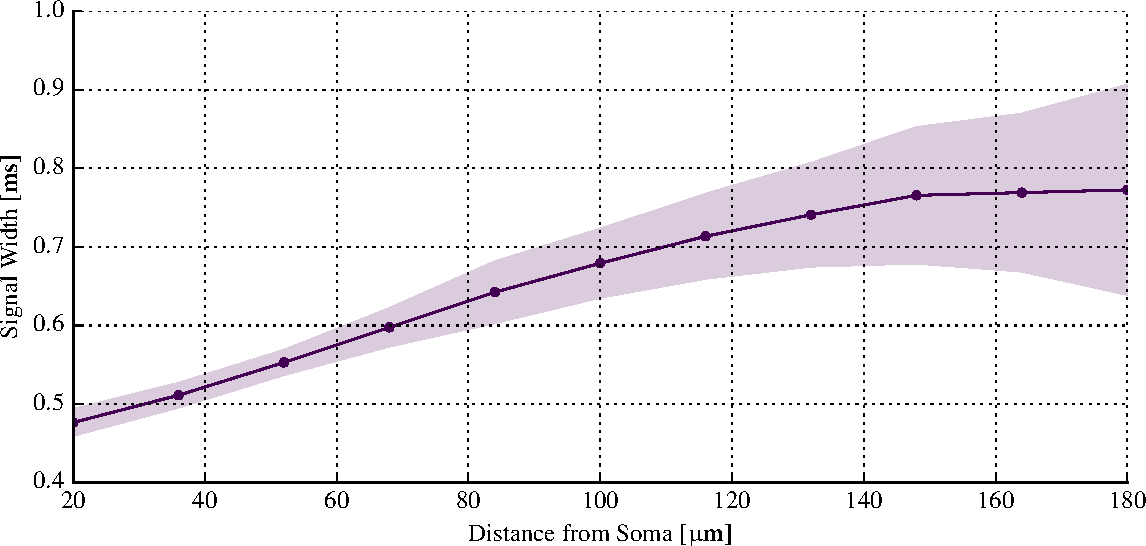
\includegraphics[width=\textwidth]{images/3_methods/3_1_reproduction/circular_spike_width_std.pdf}
\caption{Spike width over distance. Mean +/- 1 std.}
\label{fig:3_1_spike_width}
\end{figure}

\textcite{pettersen_amplitude_2008} reports a spike amplitude above $150\mu V$ at 
$20\mu m$, this does not match current findings.  
Figure \ref{fig:3_1_spike_amp} shows spike amplitude with logarithmic axes.  
(TODO: Is numbers on the power law decays necessaryy?) Although 
the data does not match \textcite{pettersen_amplitude_2008}, 
it is comparable with what is
expected in the near and far limit field of a ball and stick neuron.
In the near field the the expectation is a $1/r$ decay and in the far field
it is  $1/r^2$ or $1/r^3$ depending on distance. (TODO: Clearify this, put reference
back to theory chapter.)

\begin{figure}[thp]
\centering
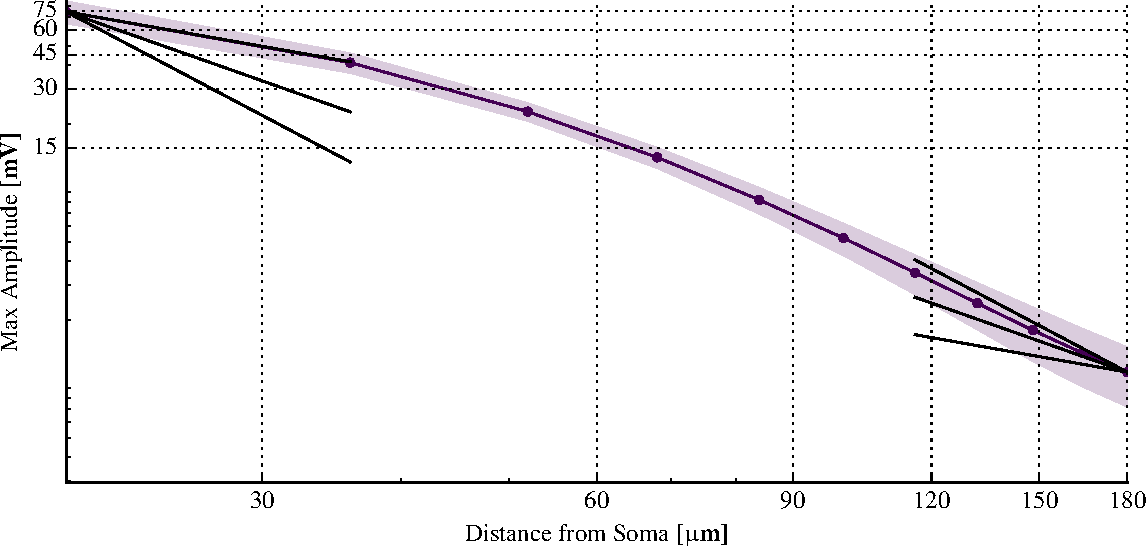
\includegraphics[width=\textwidth]{images/3_methods/3_1_reproduction/circular_spike_amp_std_log.pdf}
\caption{Spike amplitude over distance. Mean +/- 1 std. The power law
decays $1/r$, $1/r^2$ and $1/r^3$ are shown at the leftmost and rightmost
data points.}
\label{fig:3_1_spike_amp}
\end{figure}

\subsection{Discussion?}

\newpage
\section{Blue Brain}
Use the models. Write code to capture one action potential. Bursting neurons
often hav adapting action potential, what to do there. 

Have a volume of electrodes, calculate the amplitude and where they stop being 
noticable. Plot where the signal can be recoqnized. 

\section{Allen Brain Institute}

My spesific implementation of LFPy and Neuron. 

The recording site for the electrophysiological data is soma for all neuron in the data from 
Allen Brain Institute.
The currents in the dendrites are not avaiable and is modelled using a passive neuron model.
Write how the simulation is set up. 


Create convincing results that shows that the simulations are correct and can be trusted. 

Reproduction of results from \cite{pettersen2008amplitude}. 
\begin{itemize}
	\item Action potential width and amplitude is correct. 
	\item Fourier specter is correct. 
	\item Extracellular width and amplitude matches the article. 
	\item Create same plots. 
	\item Calculate the same parameters, power law?
\end{itemize}

How different are action potentials generated from the same cell. How does the "mean" spike look
from the experimental data. 

Data from Blue Brain and Allen Brain Institute. 

Allen Brain Institute Questions:
\begin{itemize}
	\item How much does the experimental spikes differ. 
\end{itemize}

\chapter{Results}
Use membrane potentials from Allen Brain Institute and Blue Brain and look at width from different cells. 



\chapter{Discussion}



\nocite{*}
\printbibliography[heading=bibintoc]

\end{document}